% Propósito: relacionar el estado físico de un oscilador con las fases de su
% posición, velocidad y aceleración.
% Origen: x/A=cos(2 pi t/T), v/(omega A)=-sin(2 pi t/T) y
% a/(omega^2 A)=-cos(2 pi t/T), ecuaciones
% \eqref{eq:u3-mas-posicion}, \eqref{eq:u3-mas-velocidad} y
% \eqref{eq:u3-mas-aceleracion}, con fase inicial igual a cero.
% Curvas teóricas normalizadas; no representan datos medidos.
% Descripción accesible: arriba se muestra una masa en el extremo positivo,
% con aceleración hacia el equilibrio. Debajo, tres gráficos normalizados
% muestran que posición y aceleración tienen signos opuestos, y que la
% velocidad es máxima al pasar por el equilibrio.
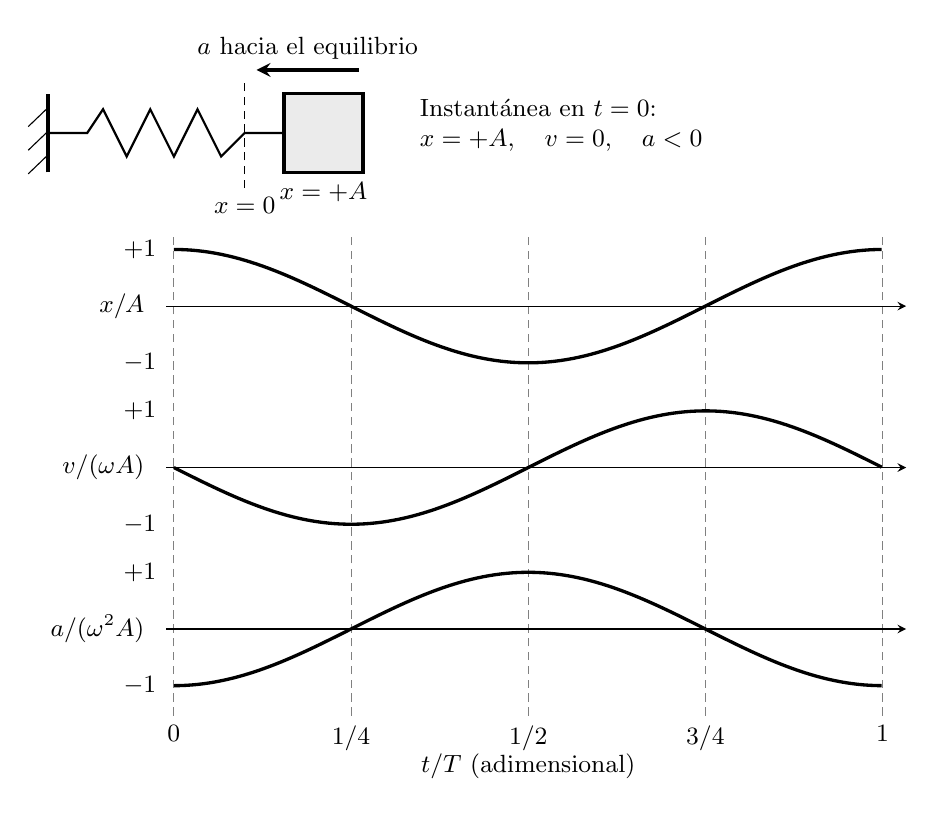
\begin{tikzpicture}[font=\small,>=stealth,x=1cm,y=1cm]
    % Instantánea física correspondiente a t=0.
    \draw[very thick] (0.55,3.75) -- (0.55,4.75);
    \foreach \y in {3.85,4.15,4.45}{
        \draw (0.30,\y-0.12) -- (0.55,\y+0.12);
    }
    \draw[thick] (0.55,4.25) -- (1.05,4.25)
        -- (1.25,4.55) -- (1.55,3.95)
        -- (1.85,4.55) -- (2.15,3.95)
        -- (2.45,4.55) -- (2.75,3.95)
        -- (3.05,4.25) -- (3.55,4.25);
    \draw[very thick,fill=black!8] (3.55,3.75) rectangle (4.55,4.75);
    \draw[densely dashed] (3.05,3.55) -- (3.05,4.95);
    \node[below] at (3.05,3.55) {\(x=0\)};
    \node[below] at (4.05,3.75) {\(x=+A\)};
    \draw[->,very thick] (4.50,5.05) -- (3.20,5.05)
        node[midway,above] {\(a\) hacia el equilibrio};
    \node[anchor=west,align=left] at (5.15,4.35)
        {Instantánea en \(t=0\):\\\(x=+A,\quad v=0,\quad a<0\)};

    % Escalas comunes de tiempo normalizado.
    \foreach \q/\lab in {0/{0},0.25/{1/4},0.5/{1/2},0.75/{3/4},1/{1}}{
        \pgfmathsetmacro{\xx}{2.15+9.0*\q}
        \draw[densely dashed,gray] (\xx,-3.15) -- (\xx,2.95);
        \node[below] at (\xx,-3.15) {\(\lab\)};
    }

    % Ejes horizontales de las tres magnitudes.
    \foreach \yy in {2.05,0,-2.05}{
        \draw[->] (2.05,\yy) -- (11.45,\yy);
    }
    \node[anchor=east] at (1.90,2.05) {\(x/A\)};
    \node[anchor=east] at (1.90,0) {\(v/(\omega A)\)};
    \node[anchor=east] at (1.90,-2.05) {\(a/(\omega^{2}A)\)};
    \node at (6.65,-3.80) {\(t/T\) (adimensional)};

    % Curvas normalizadas.
    \draw[very thick,samples=120,domain=0:1]
        plot ({2.15+9.0*\x},{2.05+0.72*cos(360*\x)});
    \draw[very thick,samples=120,domain=0:1]
        plot ({2.15+9.0*\x},{-0.72*sin(360*\x)});
    \draw[very thick,samples=120,domain=0:1]
        plot ({2.15+9.0*\x},{-2.05-0.72*cos(360*\x)});

    % Límites normalizados.
    \foreach \yy in {2.05,0,-2.05}{
        \node[anchor=east] at (2.05,\yy+0.72) {\(+1\)};
        \node[anchor=east] at (2.05,\yy-0.72) {\(-1\)};
    }
\end{tikzpicture}
